\documentclass[12pt,preprint]{aastex}

\usepackage{verbatim}
\usepackage{color}
\usepackage[normalem]{ulem} % for striking out with \sout
\usepackage{amsmath} % for boldsymbol
% A comment block

%\newcommand{\comment}[1]{}

% For color
\newcommand{\mpname}[1]{#1_color.eps}
\newcommand{\clraitoff}{red}
\newcommand{\lumblack}{(black)}
\newcommand{\lumblue}{(blue)}
\newcommand{\lumred}{(red)}
\newcommand{\vdisred}{(red-dashed curve)}
\newcommand{\vdisblue}{(blue-solid curve)}

% For bw
%\newcommand{\mpname}[1]{#1.eps}
%\newcommand{\clraitoff}{}
%\newcommand{\lumblack}{}
%\newcommand{\lumblue}{}
%\newcommand{\lumred}{}
%\newcommand{\vdisred}{(dashed curve)}
%\newcommand{\vdisblue}{(solid curve)}

\newcommand{\umag}{$u$}
\newcommand{\gmag}{$g$}
\newcommand{\rmag}{$r$}
\newcommand{\imag}{$i$}
\newcommand{\zmag}{$z$}
\newcommand{\gmr}{$g-r$}



\newcommand{\gammat}{$\gamma_T$}
\newcommand{\gammacross}{$\gamma_\times$}
\newcommand{\deltasig}{$\Delta \Sigma$}
\newcommand{\deltaplus}{$\Delta \Sigma_+$}
\newcommand{\deltacross}{$\Delta \Sigma_\times$}
\newcommand{\deltarho}{$\Delta \rho$}
\newcommand{\movr}{$M(<r)$}
\newcommand{\sigmacrit}{$\Sigma_{crit}$}

\newcommand{\photoz}{photo-z}
\newcommand{\photozs}{photo-zs}

\newcommand{\tlum}{$L^{tot}$}
\newcommand{\tngal}{$N_{gal}^{tot}$}

\newcommand{\lstarlim}{$0.4 L_*$}
\newcommand{\lvir}{$L_{200}$}
\newcommand{\lvirtot}{$L^{tot}_{200}$}
\newcommand{\mvir}{$M_{200}$}
\newcommand{\nvir}{$N_{200}$}
\newcommand{\rvirgal}{$r_{200}^{gals}$}
\newcommand{\rvirmass}{$r_{200}^{mass}$}

\newcommand{\deltamtol}{$\Delta M/\Delta L$}
\newcommand{\deltam}{$\Delta M$}
\newcommand{\deltal}{$\Delta L$}

\newcommand{\deltamvir}{$\Delta M_{200}$}
\newcommand{\deltalvir}{$\Delta L_{200}$}

\newcommand{\mtolmax}{$(\Delta M/\Delta L)_{22\mathrm{Mpc}}$}
\newcommand{\mtolasym}{$(\Delta M/\Delta L)_{asym}$}
\newcommand{\mtolvir}{$(\Delta M/\Delta L)_{200}$}
\newcommand{\bmtol}{$b^2_{M/L}$}
\newcommand{\bmtolinv}{$b^{-2}_{M/L}$}

\newcommand{\ngal}{$N_{gal}$}
\newcommand{\maxbcg}{MaxBCG}
\newcommand{\numNgalBins}{12}
\newcommand{\numLumBins}{16}

\newcommand{\tngalAperture}{2$h^{-1}$ Mpc}

\newcommand{\photo}{\texttt{PHOTO}}
\newcommand{\astrop}{\texttt{ASTRO}}
\newcommand{\mt}{\texttt{MT}}
\newcommand{\spectro}{\texttt{SPECTRO}}
\newcommand{\spectroone}{\texttt{SPECTRO1d}}
\newcommand{\spectrotwo}{\texttt{SPECTRO2d}}
\newcommand{\target}{\texttt{TARGET}}

\newcommand{\lenszmax}{0.3}
\newcommand{\lenszmin}{0.05}
\newcommand{\zmean}{0.25}

\newcommand{\photoversion}{\texttt{v5\_4}}

%\def\eone{e$_1$}
%\def\etwo{e$_2$}
\newcommand{\etan}{e$_+$}
\newcommand{\erad}{e$_\times$}
\newcommand{\eclass}{\texttt{ECLASS}}
\newcommand{\eclasscut}{-0.06}
\newcommand{\gmrcut}{0.7}

\newcommand{\hrs}{$^{\mathrm h}$}
\newcommand{\minutes}{$^{\mathrm m}$}

\newcommand{\ugriz}{$u, g, r, i, z$}
\newcommand{\polarization}{polarization}

\newcommand{\wgm}{$w_{gm}$}
\newcommand{\wgg}{$w_{gg}^p$}
\newcommand{\wmm}{$w_{mm}$}
\newcommand{\xigg}{$\xi_{gg}$}
\newcommand{\ximm}{$\xi_{mm}$}
\newcommand{\xigm}{$\xi_{gm}$}

\newcommand{\numspec}{127,001}
\newcommand{\numspecvlim}{10,277}
\newcommand{\numrand}{1,270,010}
\newcommand{\numspectot}{278,192}
\newcommand{\numvdis}{49,024}
%\newcommand{\numsource}{10,259,949}
% hirata: 
\newcommand{\nummask}{1,815,043}
\newcommand{\numTenMpc}{132,473}
\newcommand{\numThirtyMpc}{101,221}
\newcommand{\numsource}{27,912,891}

\newcommand{\numpairsTenMpc}{2,670,898,177}
\newcommand{\altnumpairsTenMpc}{2.7 billion}
\newcommand{\numpairsThirtyMpc}{14,818,082,122}
\newcommand{\altnumpairsThirtyMpc}{14.8 billion}



\newcommand{\xirmax}{$\xi_{gm}(R_{max})$}


\def\eps@scaling{1.0}% 

\newcommand{\Tsn}{$(S/N)_{size}$}
\newcommand{\fsn}{$(S/N)_{flux}$}

% stolen from the BA13 source
\newcommand{\vecg}{\mbox{\boldmath $g$}}
\newcommand{\vecD}{\mbox{\boldmath $D$}}
\newcommand{\vecQ}{\mbox{\boldmath $Q$}}
\newcommand{\matR}{\mbox{$\bf R$}}
\newcommand{\matC}{\mbox{$\bf C$}}
\newcommand{\bnabg}{ \boldsymbol{\nabla_g}}

\slugcomment{Last revision \today}
\shortauthors{Sheldon}
\shorttitle{Bayesian Shear Estimation}

\begin{document}

\title{On Bayesian Shear Estimation}

\author{
Erin S. Sheldon\altaffilmark{1}
}
\altaffiltext{1}{Brookhaven National Laboratory, Bldg 510, Upton, New York 11973}



\begin{abstract}

blah

\end{abstract}

\section{Introduction} \label{sec:intro}

intro

\section{Algorithm} \label{sec:algo}

The full algorithm is presented in \citet[][BA13]{ba13}.  There are a few basic
assumptions underlying this approach.  Following the notation in BA13:

\begin{itemize}

    \item The shear is weak, $g \ll 1$.

    \item In the limit of weak shear, only the ensemble mean shear can be
        derived from galaxy shapes.

    \item The posterior distribution of the shear derived from a large ensemble
        of galaxy images is Gaussian.


\end{itemize}

The first assumption is true under most circumstances, but will break down
along lines-of-sight near large over-densities, such as clusters of galaxies.

The second assumption follows from the first, and the fact that galaxy images
are to be used to estimate the shear: galaxies have intrinsic shapes, with
variance larger than the typical shear induced by structures in our universe.
Given this limitation, the estimation of shears from individual sources is
abandoned.  This limitation would not apply if a large set of intrinsically
round, extended sources were found.

The third point follows from the central limit theorem: if the shear is derived
from a large enough ensemble of galaxy shapes, the posterior necessarily
approaches a Gaussian.

Under these assumptions, a second-order estimator was derived for the shear,
consistent with the assumption of a Gaussian posterior.  This form is a Taylor
expansion of the logarithm of the posterior for the shear, with shear as the
expansion variable:
\begin{equation} \label{eq:pexpand}
-\ln P(\vecg | \vecD) \approx {(\rm const)} - \ln P(\vecg) - \vecg \cdot \sum_i
    \frac{\vecQ_i}{P_i}
    + \frac{1}{2} \vecg \cdot \left[ \sum_i \left(\frac{\vecQ_i \vecQ^T_i}{P_i^2}
    - \frac{\matR_i}{P_i}\right) \right] \cdot \vecg,
\end{equation}
where the terms $P_i$, $\vecQ_i$, and $\matR_i$ are 
\begin{eqnarray} \label{eq:pqrdef}
P_i     & = & P(\vecD_i | \vecg=0) \nonumber \\
\vecQ_i & = & \left. \bnabg P(\vecD_i | \vecg)\right|_{\vecg=0} \\
\matR_i & = & \left. \bnabg \bnabg P(\vecD_i | \vecg)\right|_{\vecg=0}. \nonumber
\end{eqnarray}

Prior information is key to this approach: these equations involve derivatives
of the un-lensed distribution of shapes, the prior $P$. To fully predict the
observed distribution of shapes, the un-lensed distribution of shapes must be
mathematically sheared and compared to observables.  Due to the approximations,
only derivatives near $g=0$ are required. The mean shear can be solved for and
is given by:
\begin{eqnarray} \label{eq:shdef}
\matC_g^{-1} & = & \sum_i \left(\frac{\vecQ_i \vecQ^T_i}{P_i^2} - \frac{\matR_i}{P_i}\right) \\
\bar{\vecg} & = &  \matC_g \sum_i \frac{\vecQ_i}{P_i}.
\end{eqnarray}

In practice the shape of each galaxy is not precisely known. The derivatives in
equation \ref{eq:pqrdef} are marginalized over the full likelihood distribution
for each galaxy, and these marginalized values are used in the aggregate shown
in equation \ref{eq:shdef}.  The use of strong priors on all parameters also
suppresses noise-related effects, such as the shear ``noise bias''.  

An approach to measuring non-constant shear is also given, as are third-order
tweaks to the second-order perturbations, but implementations of those ideas
are left to future work.

A full implementation, fitting to pixelized galaxy images, was not attempted in
\citet{ba13}.  The basic formalism was shown to work by generating shapes from
an analytic distribution, adding noise and shear, and recovering the underlying
shear using the second-order formula.

\section{Implementation} \label{sec:impl}

For this work a full implementation of the \citet{ba13} formalism was developed
to work with full pixelized noisy galaxy images, accounting for the point
spread function.

%Two types of models were fitted: An elliptical exponential disk model exp$(-r)$,
%and an elliptical \devauc\ profile exp$( -r^{1/4} )$.

The estimator involves integrals over the full likelihood distribution for each
galaxy.  Exploration of the likelihood surface requires a large number of model
evaluations.  As an optimization, galaxy models were approximated as sums of
Gaussians according the to the fits in \citet{HoggGMix12}.  The PSF was also
approximated using Gaussians.  This use of Gaussians for both galaxy and PSF
models facilitates analytic convolutions of the galaxy model with the PSF.
This is a faster and simpler alternative to convolutions using Fourier
transforms. While only approximate representations, the small associated error
in the shear recovery was not detectable in the simulations presented below.

A fast exponential function was used\footnote{https://github.com/herumi/fmath.
The code was translated from C++ to C by the author.} for rendering the galaxy
and PSF profiles.  Even so evaluation of the exponential function is the
bottleneck for this calculation.

A Markov Chain Monte Carlo (MCMC) was used to explore the posterior surface.
Galaxies can have a wide variety of model parameters and errors in the best-fit
parameters.  It is not straightforward to predict what the parameter errors
will be before doing the full fit.  For this reason an affine invariant MCMC
method was used, as first presented in \citet{GoodmanWeare10}.  A new C code
was developed to for this, which is available on request. The python
implementation presented in \citet{Mackey13} was used during prototyping.  For
each galaxy, 20 ``walkers'' were used in the chain, with 400 burnin steps and
200 steps used for calculations.

\section{Simulation} \label{sec:sim}

Simulated galaxy models were generated in ``ring pairs'' \citep{Nakajima2007}.
Pairs of galaxy images were generated at 90 degree offset in position
angle, to cancel shape noise.

Two types of models were generated, exponential disks and \devauc\ profiles.
The simulated PSF was a single round Gaussian with $\sigma = \sqrt{2}$ pixels
$(T=4)$.  A simple PSF was chosen so that PSF modeling was not an issue.

The un-lensed shape distribution was identical to the toy distribution used in
\cite{ba13}.  This distribution is not a good description of real galaxy
shapes, but was chosen for consistency with that work.  That distribution also
has the required property that it is twice differentiable.

The other galaxy parameters were drawn from simple distributions.  The size
parameter $T=I_{xx} + I_{yy}$ was drawn from a log-normal distribution with
scatter of 15\%.  The total flux was drawn from a log-normal with 30\% scatter.
The centroid was drawn from a Gaussian in each coordinate, with $\sigma$ of 0.2
pixels.

\section{A Note on Parametrization}

Because Gaussians were used for modeling both Galaxies and PSF, it is
convenient to parameterize objects in terms of the second moments rather than
alternative quantities such as half-life radii.  This parametrization is also
intuitive: for real images it is the unweighted second moments that are
modified by convolution with the PSF of instrument and atmosphere; the
covariance matrices simply add. Another way to put this is that it is the area
that is modified by the isotropic part of the PSF, and it is the ratio of areas
that controls the influence of the PSF on the shape of a galaxy.  The quantity
$T = I_{xx} + I_{yy}$, which is proportional to area, was chosen as a
convenient size parameter.

\section{Results} \label{sec:results}

Pairs of simulated galaxies were generated as described in \S \ref{sec:sim}. In
all cases, the galaxies were convolved with a circular Gaussian with
$\sigma_{\textrm{psf}}=\sqrt{2}$ pixels $(T_{\textrm{psf}}=4)$.

The simulated images were fit using parametrized models as presented in
\S \ref{sec:impl}.   A Gaussian was fit to a rendered, pixelized PSF model, and
the model was generated by analytically convolving the galaxy model with this
PSF model. By using a fit to the observed, pixelized PSF, the convolution by
the pixels is built in to the PSF model, thus forward modeling the full galaxy,
PSF, and pixelization.  While a single Gaussian is not the true model for a
pixelized Gaussian PSF, in practice the single Gaussian is sufficient for
the resolution of these simulations $\sigma_{\textrm{psf}}=\sqrt{2}$.  For
more a under-sample PSF this would not necessarily be the case.

Prior distributions were chosen to match exactly the true distributions used in
the simulation.  The correct model was fit in each case; i.e. when simulating
exponential disks, an exponential disk was fit.  By choosing the true priors
and model, the accuracy of the algorithm is tested without confusion with other
issues such as model bias and emprical prior determination.

\begin{figure}[p] \centering
 \centering 
 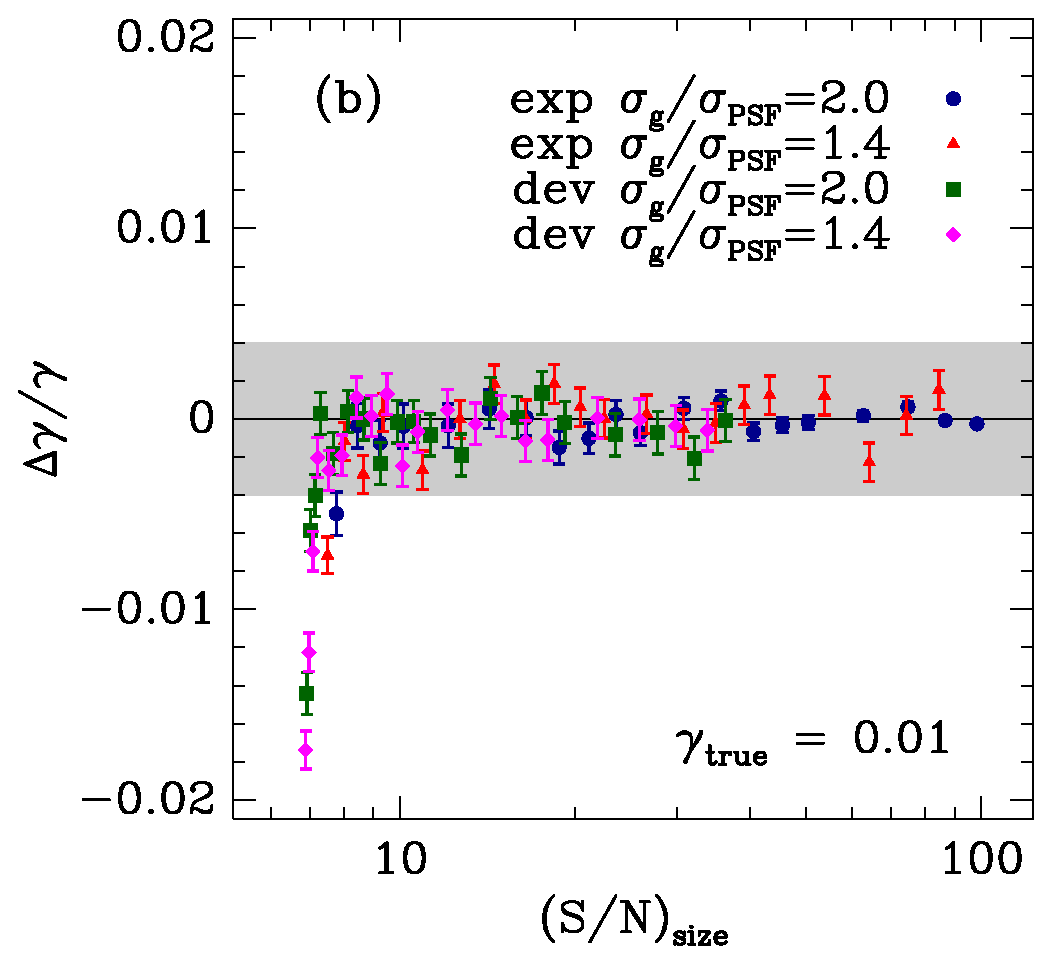
\includegraphics[scale=0.45]{figures/cbafit-geg-T-s2n.eps}
 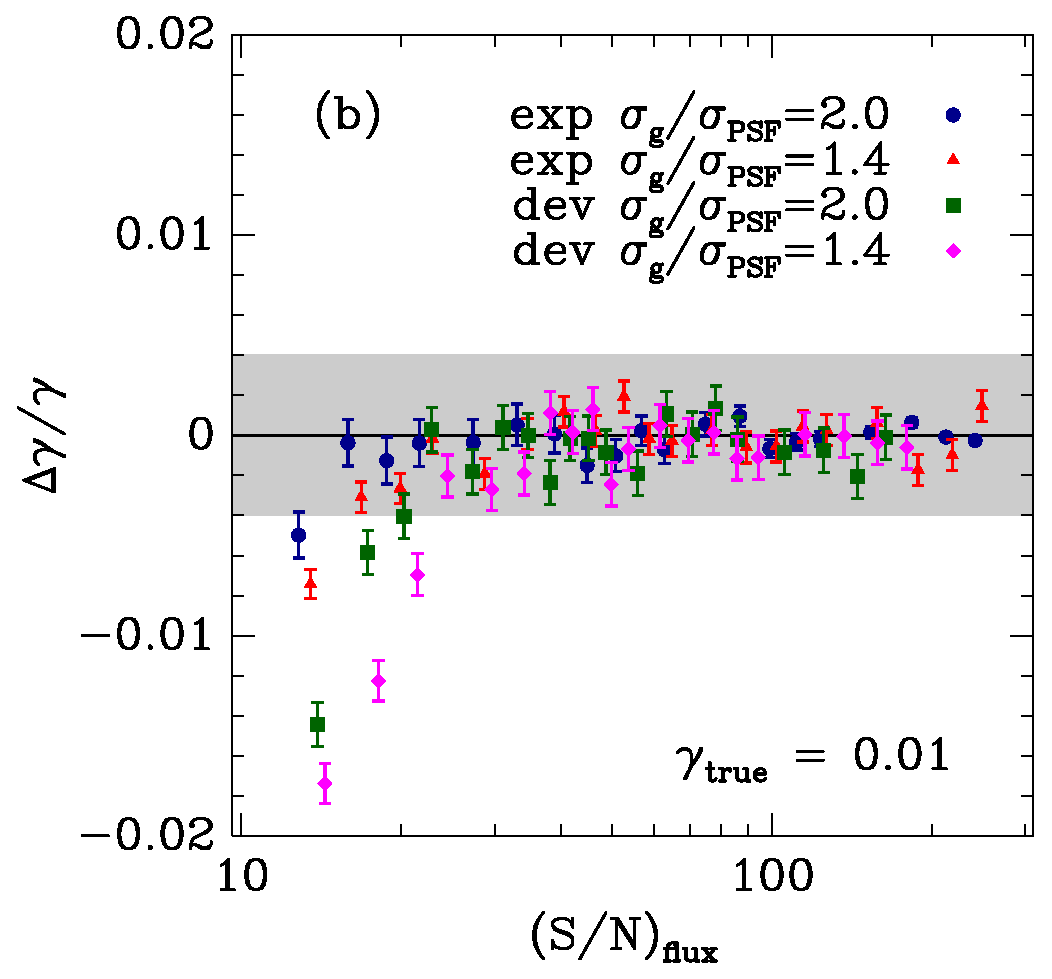
\includegraphics[scale=0.45]{figures/cbafit-geg-flux-s2n.eps}

 \caption{ Fractional bias in the recovered shear for the estimator presented
     in \cite{ba13}.  The bias is plotted as a
     function of galaxy signal-to-noise ratio (S/N), for various galaxy
     properties and two different measures of S/N.  In panel (a) is
     plotted \Tsn, where the measure of size is $T=I_{xx} + I_{yy}$.  In 
     panel (b) is plotted \fsn.  The flux and $T$ are parameters in the model
     fits, and the associated (S/N) is the ratio of best-fit value to error in
     the fit.  In each panel the fractional error is plotted for galaxies of
     different size and type, as described in the text.  As shown panel (a)
     panel, the bias depends uniquely on \Tsn\ for different galaxy types and
     sizes.  However, \fsn\ is not a sufficient descriminator for different
     galaxy types and sizes.  The \Tsn\ can be used to remove galaxies from the
     sample that will yield poor shear estimates, independent of galaxy
     properties, but not so \fsn.  For \Tsn$~ > 10$ this shear estimator meets
 the accuracy requirements for the Dark Energy Survey, shown as the gray band.
 \label{fig:fracerr}}

\end{figure}

\begin{figure}[t] \centering
 \centering 
 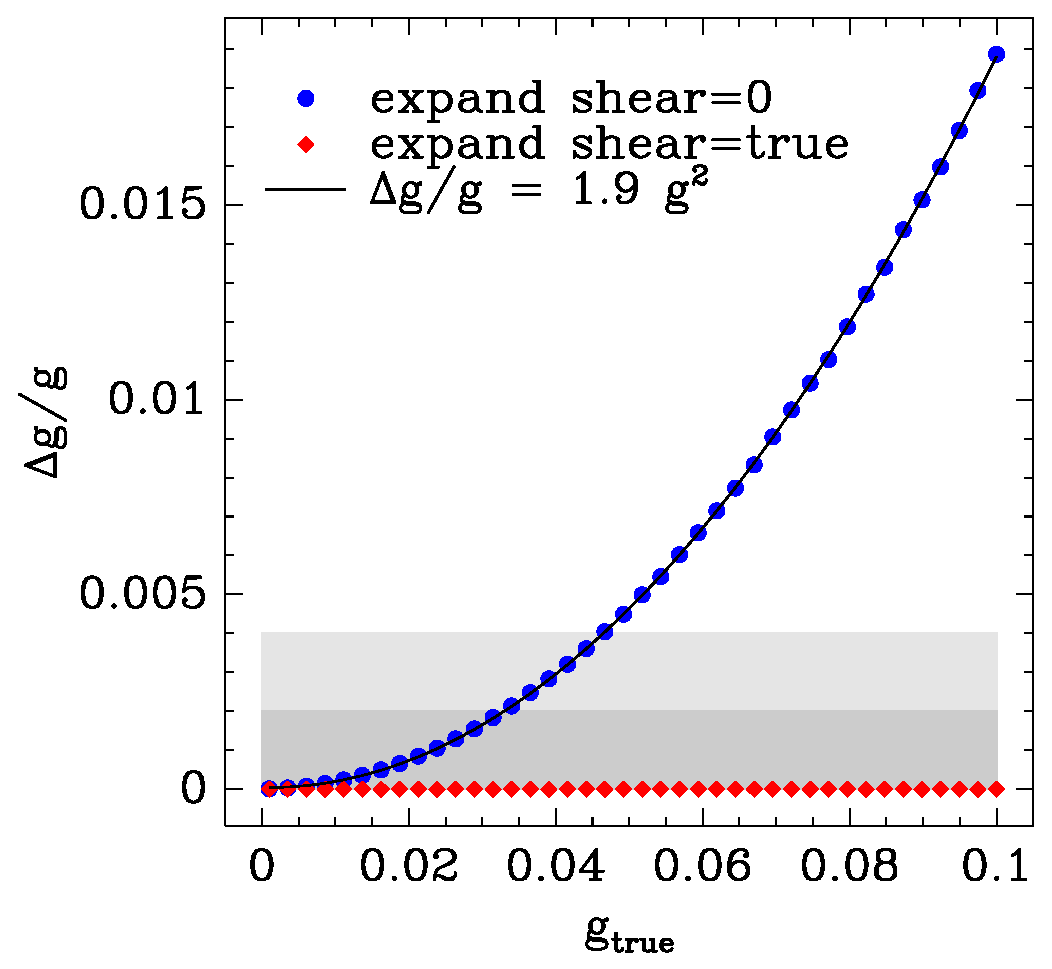
\includegraphics[scale=0.6]{figures/fracerr-vs-shear.eps}

 \caption{Fractional bias in the recovered shear as a function of true shear,
     in a zero noise simulation.  The solid curve is the best-fit quadratic
     function of the true shear.  The quadratic bias as a function of true
     shear indicates a break down of the second-order approximation presented
     in \cite{ba13}. The gray band represents the requirements for the Dark
 Energy Survey. \label{fig:nonoise}}

\end{figure}

\section{Summary} \label{sec:summary}

summary

\section*{Acknowledgments}

ES is supported by DOE grant DE-AC02-98CH10886.

Thanks to Gary Bernstein, Bob Armstrong, and Anze Slosar for many useful
discussions.

\bibliographystyle{apj}
% Bib database
\bibliography{apj-jour,astroref}

\end{document}

